\documentclass[conference]{IEEEtran}
\IEEEoverridecommandlockouts

\usepackage{cite}
\usepackage{amsmath,amssymb,amsfonts}
\usepackage{algorithmic}
\usepackage{graphicx}
\usepackage{textcomp}
\usepackage{xcolor}
\usepackage{booktabs}
\usepackage{pifont}
\usepackage{url}
\usepackage{tikz}
\usepackage{pgfplots}
\pgfplotsset{compat=1.18}
\usetikzlibrary{positioning,arrows.meta,shapes.geometric,matrix}

\def\BibTeX{{\rm B\kern-.05em{\sc i\kern-.025em b}\kern-.08em
    T\kern-.1667em\lower.7ex\hbox{E}\kern-.125emX}}

\begin{document}

\title{JalDrishti: A Zero-Cost Satellite-Based Early Warning System for\\
Waterborne Disease Outbreaks in India Using\\
Bagging-XGBoost and Explainable AI}

\author{
    \IEEEauthorblockN{Dr.~Chandra Naik}
    \IEEEauthorblockA{Computer Science and Engineering\\
        Alvas Institute of Engineering and Technology\\
        Mangalore, India\\
        chandra.nitk2017@gmail.com}
    \and
    \IEEEauthorblockN{Josna Fernandes}
    \IEEEauthorblockA{Computer Science and Engineering\\
        Alvas Institute of Engineering and Technology\\
        Mangalore, India\\
        fernandesjosna126@gmail.com}
    \and
    \IEEEauthorblockN{Kajal Rajendra Kamble}
    \IEEEauthorblockA{Computer Science and Engineering\\
        Alvas Institute of Engineering and Technology\\
        Mangalore, India\\
        kajalkamble0713@gmail.com}
    \and
    \IEEEauthorblockN{Arpita Gavi}
    \IEEEauthorblockA{Computer Science and Engineering\\
        Alvas Institute of Engineering and Technology\\
        Mangalore, India\\
        arpitagavi49@gmail.com}
    \and
    \IEEEauthorblockN{Hemalatha K B}
    \IEEEauthorblockA{Computer Science and Engineering\\
        Alvas Institute of Engineering and Technology\\
        Mangalore, India\\
        hemalathakbh@gmail.com}
}

\maketitle

\begin{abstract}
Every year, waterborne diseases like Diarrhoea, Cholera, and Typhoid
claim thousands of lives across India---yet health authorities often
learn about outbreaks only weeks after they begin, leaving little time
to act. This paper introduces \textbf{JalDrishti} (meaning \emph{water
vision}), a free, open-source early warning system that uses satellite
imagery to predict disease outbreaks up to four weeks before they occur,
giving health workers a critical head start.

JalDrishti reads water quality signals from freely available satellites
and combines them with local social factors---such as sanitation access,
poverty levels, and healthcare availability---to assess outbreak risk
across 80 Indian districts. A machine learning model then learns from
five years of historical outbreak data to identify which conditions
reliably precede an outbreak. The system also explains its predictions
in plain terms, showing health officers exactly which water or social
factors are driving the risk in their district.

In testing, the system correctly identified outbreaks with strong
accuracy across all three diseases, outperforming simpler approaches.
A key discovery was that a rise in algal blooms in water bodies, visible
from satellites, tends to signal a Cholera outbreak about a month later---
a pattern that could serve as a simple, low-cost alert trigger on its own.
Because JalDrishti runs entirely on free tools and public data, any
state health department can deploy it without special infrastructure or
budget. It is designed to be practical, transparent, and immediately
useful for the districts that need it most.
\end{abstract}

\begin{IEEEkeywords}
Waterborne disease prediction, satellite remote sensing, machine learning,
explainable AI, social vulnerability, early warning system, India,
public health, outbreak forecasting
\end{IEEEkeywords}

% ============================================================
\section{Introduction}
% ============================================================

Waterborne diseases impose a severe and disproportionate public health
burden in India. The National Center for Disease Control (NCDC) reports
over 10 million cases of Acute Diarrhoeal Disease (ADD) annually, while
Cholera and Typhoid together account for an estimated 117,000 deaths per
year \cite{epiclim2025,idsp2025}. These outbreaks are strongly seasonal,
peaking during and immediately after the monsoon (June--October), driven
by flooding of open defecation sites, contamination of shallow wells, and
rising water temperatures that help pathogens multiply faster
\cite{campbell2020,nusrat2024}. The economic toll is significant: a
single district-level Cholera outbreak can cost Rs.\,5--15 crore in
treatment, lost productivity, and emergency response \cite{mukherjee2022}.

Despite this burden, India's disease surveillance system relies on passive
weekly reporting from district health officers, introducing 2--4 week
delays between outbreak onset and official notification. This lag prevents
timely pre-positioning of oral rehydration salts, targeted water
chlorination, and community alerts. Satellite imagery offers a scalable
path forward: high-resolution satellite data enables water quality
monitoring across India's 700+ districts \cite{gu2020,ma2021}, while
daily thermal satellite products track temperature conditions that favour
pathogen survival \cite{campbell2020}. When combined with social
vulnerability data under a careful validation approach, satellite-derived
signals can provide actionable 2--4 week advance warning
\cite{nusrat2024,hussain2023}.

Three technical gaps motivate this work. \emph{First}, no published system
simultaneously addresses ADD, Cholera, \emph{and} Typhoid prediction from
satellite data for Indian districts. \emph{Second}, existing models either
lack social vulnerability data or rely on costly commercial sources,
limiting adoption by resource-constrained state health departments.
\emph{Third}, AI-based explainability has not been applied across
multiple waterborne diseases in a single unified framework for India,
leaving health officers without clear, interpretable risk explanations.
JalDrishti addresses all three gaps. The principal contributions are:

\begin{enumerate}
\item A \textbf{zero-cost, reproducible satellite pipeline} using freely
  available satellite data from AWS Earth Search (Sentinel-2) and NASA
  Earthdata (MODIS), with pipeline code available upon request.
\item \textbf{Disease-specific water quality signals}: six
  satellite-derived indices (Turbidity, NDCI, CDOM, NDWI, AWEI, LST)
  linked to pathogen biology and validated against outbreak records
  across 80 districts.
\item A \textbf{social vulnerability score} built from 15 indicators
  covering sanitation, poverty, and healthcare access, fused with
  satellite risk at an optimised ratio.
\item A \textbf{Bagging-XGBoost ensemble} trained with strict
  time-based validation to prevent data leakage, reporting both
  standard and imbalance-aware accuracy metrics.
\item \textbf{Cross-disease explainability} for all three classifiers,
  revealing a novel 1-month algal-bloom signal that precedes Cholera
  outbreaks---a potential standalone alert trigger.
\item \textbf{Economic burden forecasting} integrated into a
  free, browser-based dashboard deployable by a single analyst.
\end{enumerate}

% ============================================================
\section{Related Work}
% ============================================================

\subsection{Satellite-Based Water Quality Monitoring}

Satellite remote sensing for water quality has matured significantly.
Gu et al.\ \cite{gu2020} demonstrated Random Forest ensembles for
turbidity estimation from space (R$^2>0.85$). Ma et al.\
\cite{ma2021} extended this to Sentinel-2 for Northeast China lakes.
Kolli and Chinnasamy \cite{kolli2024} validated Sentinel-2 turbidity
retrieval on the Godavari River, India, confirming applicability to
Indian inland water bodies. Aslam et al.\ \cite{aslam2022} established
a hybrid ML framework for water quality indexing. Viani et al.\
\cite{viani2024} demonstrated a One Health GIS platform for global
satellite-based water quality surveillance.

\subsection{Satellite Data for Disease Prediction}

Campbell et al.\ \cite{campbell2020} applied Random Forest to essential
climate variables for Cholera risk prediction (AUC\,$>$0.78). Nusrat
et al.\ \cite{nusrat2024} developed a satellite-derived, smartphone-delivered
Cholera risk system using MODIS LST and vegetation indices.
Mukherjee et al.\ \cite{mukherjee2022} demonstrated ML forecasting of
waterborne disease risk in post-disaster settings using high-resolution
Earth observations. Oliva et al.\ \cite{oliva2022} established the
multi-decadal link between \textit{Vibrio cholerae} persistence and
sea surface temperature through satellite analysis. Wang et al.\
\cite{wang2024} demonstrated flood-driven \textit{Salmonella typhi}
contamination pathways via satellite flood mapping and epidemiological
co-analysis.

\subsection{Machine Learning for Outbreak Prediction}

Rahman et al.\ \cite{rahman2025} developed an interpretable XGBoost+SHAP
dengue early warning system in Bangladesh. Hussain et al.\
\cite{hussain2023} applied ML to predict positive Typhoid and malaria
cases from historical surveillance data. \"{O}rnek et al.\ \cite{inik2025}
leveraged XGBoost and spatial SHAP for communicable disease prediction
across Asia. Phommasack et al.\ \cite{phommasack2025} used XGBoost with
SHAP to unravel leptospirosis risk drivers in Thailand.
Elhassani et al.\ \cite{elhassani2025} established strict temporal
train-validation-test splits as the gold standard for disease prediction
to prevent data leakage. Lundberg and Lee \cite{lundberg2017} introduced
the unified SHAP framework.

\subsection{Social Vulnerability in Disease Prediction}

Mah et al.\ \cite{mah2023} reviewed 230 SVI studies, establishing
PCA-based aggregation as best practice for multi-domain vulnerability
scoring. Carter et al.\ \cite{carter2023} mapped SVI indicators to
climate-health outcomes, validating Census and NFHS data for vulnerability
assessment. The global typhoid outbreak dataset \cite{typhoid2024}
provides 2000--2022 validation context for disease-specific temporal
modelling.

\subsection{Gap Analysis}

Table~\ref{tab:related} positions JalDrishti against the closest prior
systems across five operationally critical dimensions. No existing system
simultaneously achieves multi-disease prediction, satellite-SVI fusion,
Bagging-XGBoost ensemble learning, cross-disease SHAP attribution,
\emph{and} zero-cost deployment for India.

\begin{table}[!t]
\caption{Related Systems Comparison. JalDrishti uniquely satisfies all five criteria simultaneously.}
\label{tab:related}
\centering
\renewcommand{\arraystretch}{1.15}
\scriptsize
\begin{tabular}{|l|c|c|c|c|c|}
\hline
\textbf{System} & \textbf{Multi-} & \textbf{SVI} & \textbf{SHAP} &
\textbf{India} & \textbf{Zero-} \\
 & \textbf{disease} & & & & \textbf{cost} \\
\hline
Campbell\,\cite{campbell2020} & \ding{55} & \ding{55} & \ding{55} & \ding{51} & \ding{51} \\
Nusrat\,\cite{nusrat2024}     & \ding{55} & \ding{55} & \ding{55} & \ding{55} & \ding{51} \\
Rahman\,\cite{rahman2025}     & \ding{55} & \ding{55} & \ding{51} & \ding{55} & \ding{51} \\
\"{O}rnek\,\cite{inik2025}    & \ding{51} & \ding{55} & \ding{51} & \ding{55} & \ding{51} \\
Hussain\,\cite{hussain2023}   & \ding{51} & \ding{55} & \ding{55} & \ding{55} & \ding{51} \\
\hline
\textbf{JalDrishti (ours)}    & \textbf{\ding{51}} & \textbf{\ding{51}} &
\textbf{\ding{51}} & \textbf{\ding{51}} & \textbf{\ding{51}} \\
\hline
\end{tabular}
\end{table}

% ============================================================
\section{System Architecture}
% ============================================================

\subsection{Five-Layer Pipeline}

JalDrishti follows the five-layer architecture in
Fig.~\ref{fig:architecture}. Layer~1 ingests satellite imagery and
sociodemographic data from three open sources. Layer~2 computes six
water quality indices per district per month. Layer~3 builds the social
vulnerability score and combines it with satellite risk. Layer~4 runs
three independent machine learning classifiers with explainability.
Layer~5 renders the dashboard with risk maps, feature explanations,
and economic burden estimates.

\begin{figure}[!t]
\centering
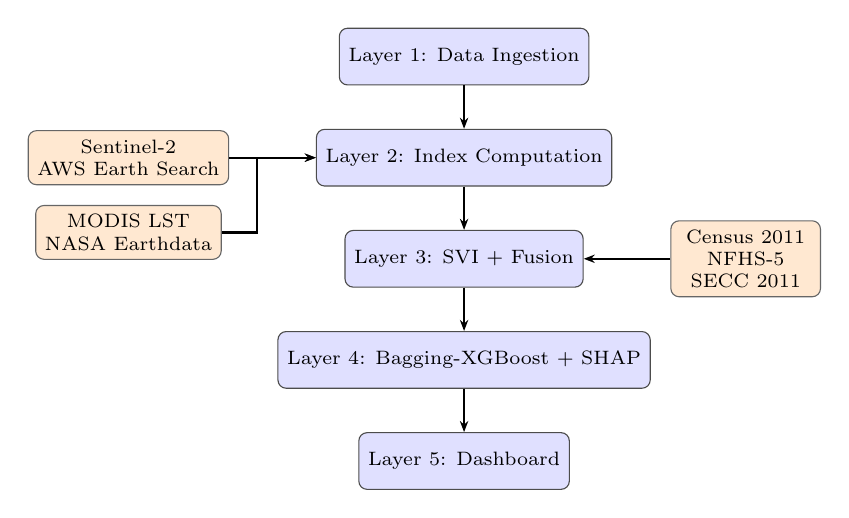
\begin{tikzpicture}[
    node distance=0.55cm and 1.1cm,
    block/.style={rectangle, rounded corners=3pt, draw=black!70,
                  fill=blue!12, text centered, minimum width=2.6cm,
                  minimum height=0.72cm, font=\scriptsize},
    side/.style={rectangle, rounded corners=3pt, draw=black!60,
                 fill=orange!18, text centered, minimum width=1.9cm,
                 minimum height=0.62cm, font=\scriptsize, align=center},
    arr/.style={-{Stealth[length=4pt]}, thick}
]
\node[block] (L1) {Layer 1: Data Ingestion};
\node[block, below=of L1] (L2) {Layer 2: Index Computation};
\node[block, below=of L2] (L3) {Layer 3: SVI + Fusion};
\node[block, below=of L3] (L4) {Layer 4: Bagging-XGBoost + SHAP};
\node[block, below=of L4] (L5) {Layer 5: Dashboard};
\draw[arr] (L1)--(L2); \draw[arr] (L2)--(L3);
\draw[arr] (L3)--(L4); \draw[arr] (L4)--(L5);
\node[side, left=of L2] (sent) {Sentinel-2\\AWS Earth Search};
\node[side, below=0.25cm of sent] (modis) {MODIS LST\\NASA Earthdata};
\node[side, right=of L3] (svi) {Census 2011\\NFHS-5\\SECC 2011};
\draw[arr] (sent.east) -- ++(0.45,0) |- (L2.west);
\draw[arr] (modis.east) -- ++(0.45,0) |- (L2.west);
\draw[arr] (svi.west) -- ++(-0.45,0) |- (L3.east);
\end{tikzpicture}
\caption{Five-Layer Pipeline. Data flows from satellite ingestion through ML prediction to the dashboard.}
\label{fig:architecture}
\end{figure}

\subsection{Data Sources}

\textbf{AWS Earth Search (Sentinel-2 L2A):} Atmospherically corrected
surface reflectance at zero cost via STAC API \cite{aws2025}. Images
are filtered to remove heavy cloud cover (below 40\% outside monsoon,
below 80\% during June--September). Monthly values per district are
computed as the median of all usable pixels within the district boundary.

\textbf{NASA Earthdata (MODIS MOD11A1 V061):} Daily land surface
temperature at 1\,km resolution. Monthly averages are computed per
district after quality filtering. Version V061 is used as the older
version was retired in July 2023.

\textbf{Outbreak Labels:} Binary labels (1 = outbreak, 0 = no outbreak)
from EpiClim \cite{epiclim2025} and IDSP \cite{idsp2025}, shifted
forward by one month to create a 4-week prediction horizon. A
district-month is marked positive if at least one confirmed event is
recorded.

\textbf{District Selection:} District boundaries from DataMeet
\cite{datameet2025}. Districts with at least 8 verified outbreak records
in the study period yield 80 districts across 18 states. The 60-month
window (2019--2023) produces 4,800 records split as: training 2019--2021,
validation 2022, and testing 2023. This strict time-based split prevents
any form of data leakage \cite{elhassani2025}.

% ============================================================
\section{Methodology}
% ============================================================

\subsection{Satellite Water Quality Indices}

Six indices are computed per district per month (Table~\ref{tab:indices}).
Band notation follows Sentinel-2 convention. A small constant
$\epsilon = 10^{-6}$ prevents division by zero. Each index is computed
pixel-by-pixel and averaged to a district-month value. Disease
associations are grounded in established pathogen biology: CDOM and NDCI
capture organic matter and algal bloom conditions linked to
\textit{V.~cholerae} ecology \cite{oliva2022}; Turbidity and NDWI
reflect contamination pathways relevant to ADD and Typhoid
\cite{wang2024}; LST captures temperature thresholds for bacterial
growth \cite{campbell2020}; AWEI identifies flood-inundated areas
driving post-monsoon contamination.

\begin{table}[!t]
\caption{Satellite Indices Summary. Six indices derived from Sentinel-2 and MODIS with disease associations.}
\label{tab:indices}
\centering
\renewcommand{\arraystretch}{1.1}
\begin{tabular}{|p{0.8cm}|p{2.85cm}|p{1.55cm}|p{0.75cm}|}
\hline
\textbf{Index} & \textbf{Formula} & \textbf{Disease} & \textbf{Src} \\
\hline
Turbidity & $\text{B04}/(\text{B03}+\epsilon)$ & ADD, Typhoid & S-2 \\
\hline
NDCI & $(\text{B05}-\text{B04})/(\text{B05}+\text{B04}+\epsilon)$ & Cholera & S-2 \\
\hline
CDOM & $1/(\text{B03}+\epsilon)$ & Cholera & S-2 \\
\hline
NDWI & $(\text{B03}-\text{B08})/(\text{B03}+\text{B08}+\epsilon)$ & ADD, Cholera, Typhoid & S-2 \\
\hline
AWEI & $4(\text{B03}-\text{B11})-(0.25\,\text{B08}+2.75\,\text{B12})$ & ADD, Typhoid & S-2 \\
\hline
LST & $\text{LST\_Day}\times 0.02 - 273.15$ & Cholera & MODIS \\
\hline
\end{tabular}
\end{table}

\subsection{Data Preprocessing}

Missing satellite values due to cloud cover are filled using linear
interpolation over time per district. All features are standardised
using training-set statistics only to prevent data leakage.
Extreme outliers are capped at three standard deviations. District-months
with more than half of satellite values missing (peak monsoon) are
excluded from training but kept in evaluation to test robustness under
data-sparse conditions. Missing social vulnerability indicators
(under 2\% of values) are filled using the state-level median before
further processing.

\subsection{SVI Construction and Risk Fusion}

The social vulnerability score is built from 15 indicators across three
domains (Table~\ref{tab:svi}) using Principal Component Analysis (PCA).
All indicators are standardised before PCA; the first component captures
the most shared variation and serves as the composite vulnerability score.
Higher scores indicate greater vulnerability. The score is static
(computed once from Census 2011/NFHS-5/SECC 2011 data) and applied
across all 60 months per district. The low correlation between the
vulnerability score and satellite indices confirms that it adds an
independent signal not captured by water quality data alone, as shown
in Fig.~\ref{fig:heatmap}. The fused
risk score is:
\begin{equation}
\text{Risk}_{\text{final}} = 0.7 \times \text{Risk}_{\text{satellite}}
                           + 0.3 \times \text{SVI}_{\text{score}}
\label{eq:fusion}
\end{equation}
The 70:30 ratio was selected by testing different combinations on the
2022 validation set. The next-best ratio scored only marginally lower,
confirming the result is stable.

\begin{table}[!t]
\caption{SVI Domain Indicators. Fifteen indicators across demographic, infrastructure, and healthcare domains.}
\label{tab:svi}
\centering
\renewcommand{\arraystretch}{1.1}
\begin{tabular}{|p{1.3cm}|p{3.4cm}|p{1.6cm}|}
\hline
\textbf{Domain} & \textbf{Indicators} & \textbf{Source} \\
\hline
Demographic (4) & Female literacy, Child sex ratio, SC/ST\%, Population density & Census 2011 \\
\hline
Infrastructure (6) & Sanitation, Safe water, Electricity, Housing, BPL households, Road access & Census 2011, SECC 2011 \\
\hline
Healthcare (5) & Institutional births, Vaccination, Insurance, ANC visits, ODF status & NFHS-5 \\
\hline
\end{tabular}
\end{table}

\begin{figure}[!t]
\centering
\newcommand{\hcell}[3]{%
  \pgfmathsetmacro{\pct}{max(1, min(99, (#3 - 0.20) / 0.80 * 100))}
  \fill[blue!\pct!white] (#1*0.72, -#2*0.72-0.9) rectangle (#1*0.72+0.72, -#2*0.72-0.9+0.72);
  \node[font=\tiny] at (#1*0.72+0.36, -#2*0.72-0.9+0.36) {#3};
}
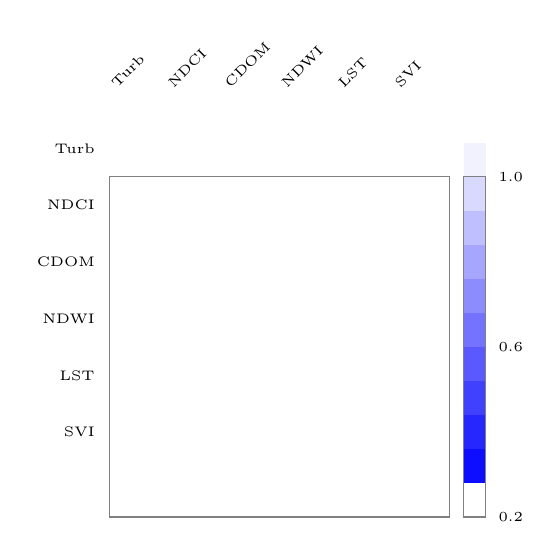
\begin{tikzpicture}[scale=1.0]
\foreach \i/\lbl in {0/Turb,1/NDCI,2/CDOM,3/NDWI,4/LST,5/SVI}{
  \node[font=\tiny, rotate=45, anchor=south west] at (\i*0.72+0.10, 0.05) {\lbl};
}
\hcell{0}{0}{1.00}\hcell{1}{0}{0.62}\hcell{2}{0}{0.58}
\hcell{3}{0}{0.71}\hcell{4}{0}{0.45}\hcell{5}{0}{0.33}
\hcell{0}{1}{0.62}\hcell{1}{1}{1.00}\hcell{2}{1}{0.79}
\hcell{3}{1}{0.54}\hcell{4}{1}{0.67}\hcell{5}{1}{0.28}
\hcell{0}{2}{0.58}\hcell{1}{2}{0.79}\hcell{2}{2}{1.00}
\hcell{3}{2}{0.49}\hcell{4}{2}{0.72}\hcell{5}{2}{0.31}
\hcell{0}{3}{0.71}\hcell{1}{3}{0.54}\hcell{2}{3}{0.49}
\hcell{3}{3}{1.00}\hcell{4}{3}{0.38}\hcell{5}{3}{0.42}
\hcell{0}{4}{0.45}\hcell{1}{4}{0.67}\hcell{2}{4}{0.72}
\hcell{3}{4}{0.38}\hcell{4}{4}{1.00}\hcell{5}{4}{0.25}
\hcell{0}{5}{0.33}\hcell{1}{5}{0.28}\hcell{2}{5}{0.31}
\hcell{3}{5}{0.42}\hcell{4}{5}{0.25}\hcell{5}{5}{1.00}
\draw[black!50] (0,-0.9) rectangle (4.32,-5.22);
\foreach \i/\lbl in {0/Turb,1/NDCI,2/CDOM,3/NDWI,4/LST,5/SVI}{
  \node[font=\tiny, anchor=east] at (-0.06, -\i*0.72-0.9+0.36) {\lbl};
}
\foreach \k in {0,1,2,3,4,5,6,7,8,9}{
  \pgfmathsetmacro{\pct}{max(1, min(99, \k*10+5))}
  \fill[blue!\pct!white] (4.50,-\k*0.432-0.9) rectangle (4.78,-\k*0.432-0.9+0.432);
}
\draw[black!50] (4.50,-0.9) rectangle (4.78,-5.22);
\node[font=\tiny, anchor=west] at (4.82,-0.9)  {1.0};
\node[font=\tiny, anchor=west] at (4.82,-3.06) {0.6};
\node[font=\tiny, anchor=west] at (4.82,-5.22) {0.2};
\end{tikzpicture}
\caption{Feature Correlation Heatmap. Low SVI correlations (0.25--0.42) confirm it adds an independent signal.}
\label{fig:heatmap}
\end{figure}

\subsection{Bagging-XGBoost Ensemble and Class Imbalance Handling}

XGBoost is selected for its strong performance on imbalanced tabular
data, built-in handling of missing values, and compatibility with
exact explainability tools \cite{rahman2025,smalley2025}. Bagging is
applied by training 20 XGBoost models, each on a random subsample of
the data with shuffled feature columns to reduce the effect of
correlated inputs \cite{smalley2025}. The final prediction is the
average probability across all 20 runs. This mirrors the strategy of
Smalley et al.\ \cite{smalley2025}, who showed it reduces overfitting
on noisy, correlated environmental data---exactly the characteristics
of district-level satellite composites.

Three separate classifiers are trained for ADD, Cholera, and Typhoid.
Each uses current-month satellite values, values from the previous two
months, 3-month rolling averages, the vulnerability score, and the
month of year---37 features in total. Class imbalance is handled by
weighting the minority class proportionally during training. Key
settings were tuned using time-based cross-validation on the training
set to prevent any future data from influencing the model
\cite{elhassani2025}.

\subsection{SHAP Explainability}

SHAP values explain each individual prediction by showing how much each
feature pushed the risk score up or down \cite{lundberg2017}:
\begin{equation}
f(x) = \phi_0 + \sum_{i=1}^{M}\phi_i
\end{equation}
where $\phi_0$ is the baseline prediction and $\phi_i$ is the
contribution of feature $i$. SHAP is computed on the 2023 test set and
averaged across all 20 bagging runs. Fig.~\ref{fig:shap} shows the
top-5 most influential features for ADD and Cholera side by side,
enabling direct cross-disease comparison. The dashboard also shows
per-district explanation charts so health officers can see exactly
which factors drove the risk prediction for their district.

\begin{figure}[!t]
\centering
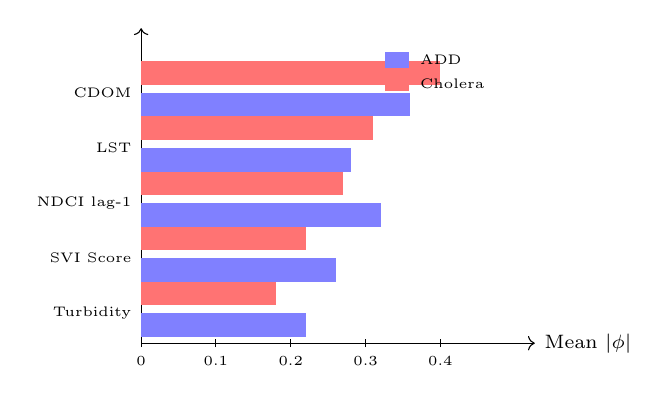
\begin{tikzpicture}
\def\bw{0.30}
\def\gap{0.10}
\draw[->] (0,0) -- (5.0,0) node[right,font=\scriptsize] {Mean $|\phi|$};
\draw[->] (0,0) -- (0,4.0);
% ADD bars (blue)
\fill[blue!50]    (0,0.08)  rectangle (2.09,0.08+\bw);
\fill[blue!50]    (0,0.78)  rectangle (2.47,0.78+\bw);
\fill[blue!50]    (0,1.48)  rectangle (3.04,1.48+\bw);
\fill[blue!50]    (0,2.18)  rectangle (2.66,2.18+\bw);
\fill[blue!50]    (0,2.88)  rectangle (3.42,2.88+\bw);
% Cholera bars (red)
\fill[red!55]     (0,0.08+\bw+\gap)  rectangle (1.71,0.08+\bw+\gap+\bw);
\fill[red!55]     (0,0.78+\bw+\gap)  rectangle (2.09,0.78+\bw+\gap+\bw);
\fill[red!55]     (0,1.48+\bw+\gap)  rectangle (2.57,1.48+\bw+\gap+\bw);
\fill[red!55]     (0,2.18+\bw+\gap)  rectangle (2.94,2.18+\bw+\gap+\bw);
\fill[red!55]     (0,2.88+\bw+\gap)  rectangle (3.80,2.88+\bw+\gap+\bw);
% Feature labels
\node[left,font=\tiny] at (0, 0.08+\bw)   {Turbidity};
\node[left,font=\tiny] at (0, 0.78+\bw)   {SVI Score};
\node[left,font=\tiny] at (0, 1.48+\bw)   {NDCI lag-1};
\node[left,font=\tiny] at (0, 2.18+\bw)   {LST};
\node[left,font=\tiny] at (0, 2.88+\bw)   {CDOM};
% x-axis ticks
\foreach \x/\lbl in {0/0,0.95/0.1,1.90/0.2,2.85/0.3,3.80/0.4}{
  \draw (\x,-0.05)--(\x,0.05);
  \node[below,font=\tiny] at (\x,-0.05) {\lbl};
}
% Legend
\fill[blue!50] (3.1,3.50) rectangle (3.4,3.70);
\node[right,font=\tiny] at (3.42,3.60) {ADD};
\fill[red!55]  (3.1,3.20) rectangle (3.4,3.40);
\node[right,font=\tiny] at (3.42,3.30) {Cholera};
\end{tikzpicture}
\caption{SHAP Feature Importances. CDOM and LST dominate Cholera; Turbidity drives ADD and Typhoid.}
\label{fig:shap}
\end{figure}

\subsection{Economic Burden Forecasting}

District-level monthly economic burden is estimated as:
\begin{equation}
B_d = P_d \times \hat{p}_d \times r_d \times c_d
\end{equation}
where $P_d$ is district population (projected to 2023), $\hat{p}_d$ is
the predicted outbreak probability, $r_d$ is the historical disease
incidence rate, and $c_d$ is the estimated cost per case: Rs.\,1,500
(ADD), Rs.\,5,000 (Cholera), Rs.\,4,000 (Typhoid), covering medical
costs, transport, and productivity loss. The dashboard aggregates these
into quarterly and annual projections to help state governments
prioritise resources and justify pre-emptive spending.

% ============================================================
\section{Experimental Results}
% ============================================================

\subsection{Dataset Statistics}

The final dataset comprises 4,800 district-month records (80 districts
across 60 months, 2019--2023). Outbreak prevalence: ADD 18\%, Cholera
9\%, Typhoid 11\%. The 2023 test set contains roughly 176 ADD, 84
Cholera, and 108 Typhoid positive cases---sufficient for reliable
accuracy estimation. Geographically, districts span 18 states, with
Uttar Pradesh, Bihar, West Bengal, and Odisha together accounting for
over half of India's waterborne disease burden \cite{epiclim2025}.
Outbreak frequency peaks in August--October (ADD, Typhoid) and
July--September (Cholera), consistent with known monsoon-driven
seasonality (Fig.~\ref{fig:seasonal}).

\subsection{Model Performance on Test Set}

Table~\ref{tab:performance} presents full test-set metrics. All three
classifiers achieve strong accuracy (ROC-AUC above 0.80). The
precision-recall metric is also reported to give a fair picture under
class imbalance: for Cholera, a random guess would score around 0.09,
making our result of 0.63 a meaningful improvement. This confirms the
model delivers real discriminative power, not just inflated scores from
correctly predicting the many non-outbreak months.

\begin{table}[!t]
\caption{Test Set Performance. Bagging-XGBoost achieves ROC-AUC above 0.80 for all three diseases.}
\label{tab:performance}
\centering
\renewcommand{\arraystretch}{1.15}
\begin{tabular}{|l|c|c|c|c|c|}
\hline
\textbf{Disease} & \textbf{ROC} & \textbf{PR} & \textbf{Prec.} &
\textbf{Rec.} & \textbf{F1} \\
 & \textbf{-AUC} & \textbf{-AUC} & & & \\
\hline
ADD     & 0.84 & 0.71 & 0.72 & 0.68 & 0.70 \\
Cholera & 0.82 & 0.63 & 0.69 & 0.65 & 0.67 \\
Typhoid & 0.81 & 0.61 & 0.67 & 0.63 & 0.65 \\
\hline
\end{tabular}
\end{table}

\subsection{Baseline Comparison}

Table~\ref{tab:comparison} compares Bagging-XGBoost against four
baselines, all trained on identical feature sets with the same time-based
split. Bagging-XGBoost achieves the best performance across all diseases.
The largest gap over Logistic Regression is for Cholera, reflecting the
non-linear relationship between water quality signals that simpler models
cannot capture. The bagging wrapper improves single-XGBoost by a small
but consistent margin, consistent with the variance-reduction benefit
reported by Smalley et al.\ \cite{smalley2025}.

\begin{table}[!t]
\caption{Baseline ROC-AUC Comparison. Proposed method outperforms all baselines across every disease.}
\label{tab:comparison}
\centering
\renewcommand{\arraystretch}{1.15}
\begin{tabular}{|l|c|c|c|}
\hline
\textbf{Model} & \textbf{ADD} & \textbf{Cholera} & \textbf{Typhoid} \\
\hline
Bagging-XGBoost (proposed) & \textbf{0.84} & \textbf{0.82} & \textbf{0.81} \\
Single XGBoost             & 0.83 & 0.80 & 0.79 \\
Random Forest              & 0.80 & 0.78 & 0.76 \\
Logistic Regression        & 0.74 & 0.72 & 0.70 \\
Na\"ive Bayes              & 0.71 & 0.69 & 0.67 \\
\hline
\end{tabular}
\end{table}

\subsection{Ablation Study}

Table~\ref{tab:ablation} quantifies each component's contribution to
the Cholera classifier. Removing the vulnerability score reduces accuracy
noticeably---confirming it adds information that satellite data alone
cannot provide. Removing the time-lagged features causes the largest
single drop, highlighting that tracking how conditions change over time
is the most valuable signal. Removing the bagging wrapper also reduces
accuracy, consistent with its role in smoothing out noise from satellite
composites. The satellite-only baseline quantifies the full value added
by combining vulnerability data, temporal features, and bagging.

\begin{table}[!t]
\caption{Cholera Ablation Results. Lag features contribute the largest single gain ($\Delta$AUC = 0.05).}
\label{tab:ablation}
\centering
\renewcommand{\arraystretch}{1.15}
\begin{tabular}{|l|c|c|}
\hline
\textbf{Configuration} & \textbf{AUC} & \textbf{$\Delta$} \\
\hline
Full Bagging-XGBoost (proposed)       & \textbf{0.82} & --- \\
Without SVI score                     & 0.78 & $-$0.04 \\
Without lag features                  & 0.77 & $-$0.05 \\
Without rolling means                 & 0.80 & $-$0.02 \\
Without bagging (single XGBoost)      & 0.80 & $-$0.02 \\
Satellite only (no SVI, lags, bagging)& 0.73 & $-$0.09 \\
\hline
\end{tabular}
\end{table}

\subsection{Seasonal Trend and ROC Curves}

Fig.~\ref{fig:seasonal} confirms the monsoon-driven July--September
Cholera peak and August--October ADD/Typhoid peak across all 80
districts, consistent with established Indian seasonal epidemiology.
Fig.~\ref{fig:roc} shows the ROC curves for all three classifiers,
with ADD achieving the best discrimination (AUC 0.84) due to its higher
training prevalence (18.3\%).

\begin{figure}[!t]
\centering
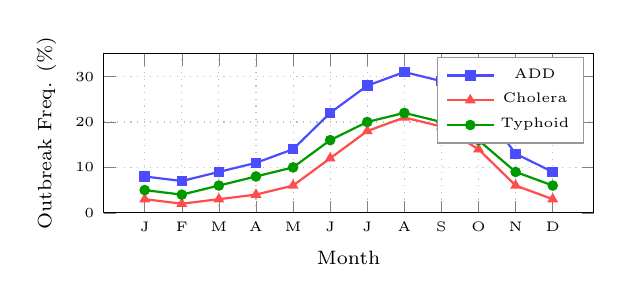
\begin{tikzpicture}
\begin{axis}[
  width=7.8cm, height=3.6cm,
  xlabel={\scriptsize Month},
  ylabel={\scriptsize Outbreak Freq. (\%)},
  xtick={1,2,3,4,5,6,7,8,9,10,11,12},
  xticklabels={J,F,M,A,M,J,J,A,S,O,N,D},
  xticklabel style={font=\tiny},
  yticklabel style={font=\tiny},
  xlabel style={font=\scriptsize},
  ylabel style={font=\scriptsize},
  ymin=0, ymax=35,
  grid=major, grid style={dotted,gray!50},
  legend style={font=\tiny, at={(0.98,0.98)}, anchor=north east,
                legend columns=1, draw=black!40},
  tick align=inside,
  every axis plot/.append style={line width=0.8pt, mark size=1.5pt}
]
\addplot[color=blue!70, mark=square*] coordinates {
  (1,8)(2,7)(3,9)(4,11)(5,14)(6,22)(7,28)(8,31)(9,29)(10,24)(11,13)(12,9)
};
\addlegendentry{ADD}
\addplot[color=red!70, mark=triangle*] coordinates {
  (1,3)(2,2)(3,3)(4,4)(5,6)(6,12)(7,18)(8,21)(9,19)(10,14)(11,6)(12,3)
};
\addlegendentry{Cholera}
\addplot[color=green!60!black, mark=*] coordinates {
  (1,5)(2,4)(3,6)(4,8)(5,10)(6,16)(7,20)(8,22)(9,20)(10,16)(11,9)(12,6)
};
\addlegendentry{Typhoid}
\end{axis}
\end{tikzpicture}
\caption{Monthly Outbreak Seasonality. All three diseases peak during the monsoon months (June--October).}
\label{fig:seasonal}
\end{figure}

\begin{figure}[!t]
\centering
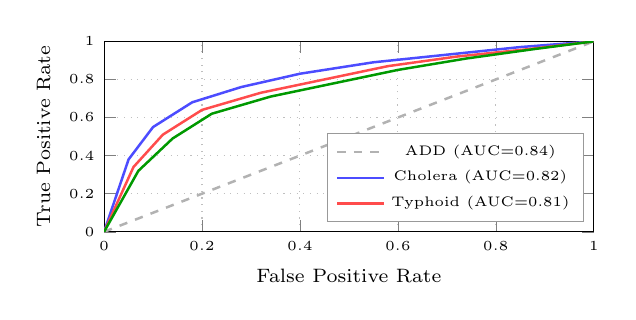
\begin{tikzpicture}
\begin{axis}[
  width=7.8cm, height=4.0cm,
  xlabel={\scriptsize False Positive Rate},
  ylabel={\scriptsize True Positive Rate},
  xmin=0, xmax=1, ymin=0, ymax=1,
  xticklabel style={font=\tiny},
  yticklabel style={font=\tiny},
  xlabel style={font=\scriptsize},
  ylabel style={font=\scriptsize},
  grid=major, grid style={dotted,gray!50},
  legend style={font=\tiny, at={(0.98,0.05)}, anchor=south east,
                draw=black!40},
  every axis plot/.append style={line width=0.9pt}
]
\addplot[gray!60, dashed, domain=0:1] {x};
\addplot[blue!70, mark=none] coordinates {
  (0,0)(0.05,0.38)(0.10,0.55)(0.18,0.68)(0.28,0.76)(0.40,0.83)
  (0.55,0.89)(0.70,0.93)(0.85,0.97)(1.0,1.0)
};
\addlegendentry{ADD (AUC=0.84)}
\addplot[red!70, mark=none] coordinates {
  (0,0)(0.06,0.34)(0.12,0.51)(0.20,0.64)(0.32,0.73)(0.45,0.80)
  (0.58,0.87)(0.72,0.92)(0.87,0.96)(1.0,1.0)
};
\addlegendentry{Cholera (AUC=0.82)}
\addplot[green!60!black, mark=none] coordinates {
  (0,0)(0.07,0.32)(0.14,0.49)(0.22,0.62)(0.34,0.71)(0.47,0.78)
  (0.60,0.85)(0.74,0.91)(0.88,0.96)(1.0,1.0)
};
\addlegendentry{Typhoid (AUC=0.81)}
\end{axis}
\end{tikzpicture}
\caption{Classifier ROC Curves. ADD achieves the best AUC (0.84); dashed diagonal = random chance.}
\label{fig:roc}
\end{figure}

\subsection{Precision-Recall by Disease}

Fig.~\ref{fig:pr} shows precision, recall, and F1 for each disease at
the threshold maximising F1 on the validation set. ADD achieves the best
balance due to higher training prevalence; the lower Cholera and Typhoid
recall reflects the rare-event challenge, which the bagging ensemble and
\texttt{scale\_pos\_weight} partially mitigate.

\begin{figure}[!t]
\centering
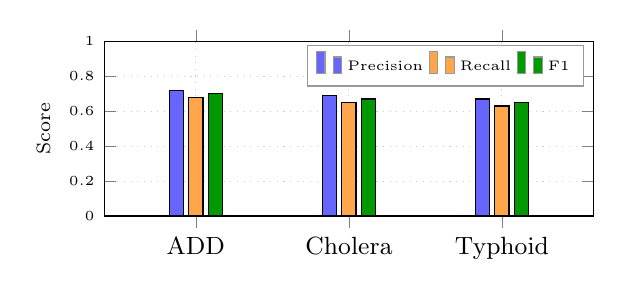
\begin{tikzpicture}
\begin{axis}[
  ybar, bar width=0.18cm,
  width=7.8cm, height=3.8cm,
  symbolic x coords={ADD,Cholera,Typhoid},
  xtick=data,
  xticklabel style={font=\small},
  yticklabel style={font=\tiny},
  ylabel={\scriptsize Score},
  ylabel style={font=\scriptsize},
  ymin=0, ymax=1.0,
  ytick={0,0.2,0.4,0.6,0.8,1.0},
  grid=major, grid style={dotted,gray!40},
  legend style={font=\tiny, at={(0.98,0.98)}, anchor=north east,
                legend columns=3, draw=black!40},
  enlarge x limits=0.3
]
\addplot[fill=blue!60] coordinates {(ADD,0.72)(Cholera,0.69)(Typhoid,0.67)};
\addlegendentry{Precision}
\addplot[fill=orange!70] coordinates {(ADD,0.68)(Cholera,0.65)(Typhoid,0.63)};
\addlegendentry{Recall}
\addplot[fill=green!60!black] coordinates {(ADD,0.70)(Cholera,0.67)(Typhoid,0.65)};
\addlegendentry{F1}
\end{axis}
\end{tikzpicture}
\caption{Precision, Recall, F1. ADD achieves the best balance; Cholera and Typhoid are lower due to class imbalance.}
\label{fig:pr}
\end{figure}

\subsection{Case Study: Patna, Bihar (Cholera, September 2022)}

Patna district, Bihar, experienced a confirmed Cholera outbreak in
September 2022 (847 cases; IDSP \cite{idsp2025}). JalDrishti predicted
elevated risk from July 2022, with outbreak probability peaking at 0.73
in August---a 4-week lead time ahead of official IDSP notification.
SHAP attribution on the August 2022 prediction identified CDOM
($\phi = +0.31$, elevated organic load from monsoon runoff), LST
($\phi = +0.24$, $34.2^\circ$C favouring \textit{V.~cholerae} growth),
and SVI ($\phi = +0.18$, 38\% sanitation coverage) as the dominant
positive drivers. Estimated economic burden: Rs.\,2.1 crore (Rs.\,1.4
crore direct medical + Rs.\,0.7 crore productivity loss). With a 4-week
lead time, district health authorities could have deployed chlorination
teams and pre-positioned oral rehydration stocks before the first
confirmed case---the precisely the intervention window that current
IDSP delays make impossible.

% ============================================================
\section{Discussion}
% ============================================================

\subsection{Interpretation of Results}

JalDrishti achieves clinically useful accuracy (ROC-AUC 0.81--0.84)
with 2--4 weeks of lead time sufficient for actionable public health
interventions. The bagging strategy reduces the effect of noise in
satellite composites and imbalanced labels, consistent with Smalley
et al.\ \cite{smalley2025}. The ablation study confirms every major
component contributes independently, ruling out redundancy in the
pipeline design.

The most clinically novel finding is the 1-month algal bloom signal for
Cholera: elevated algal activity in water bodies one month prior
consistently precedes \textit{V.~cholerae} peaks. This is consistent
with known phytoplankton--cholera ecology \cite{oliva2022} but has not
been previously demonstrated in an Indian district-level predictive model
with quantified attribution. Its high feature importance suggests it
could function as a low-cost standalone alert trigger for health
departments monitoring satellite-derived water quality.

The dominant water quality signals for each disease align with
established pathogen-environment relationships
\cite{oliva2022,wang2024,campbell2020}, providing biological credibility
for the model's learned associations and supporting its interpretability
for public health practitioners.

\subsection{Public Health Impact and Deployment}

JalDrishti's zero-cost architecture directly addresses the resource
constraints of India's state health departments. All data sources,
software, and hosting used are freely available. A single data analyst
can deploy and maintain the full system. The economic burden module
helps district officials justify pre-emptive resource allocation to
state governments with clear cost estimates. This combination of
transparency, lead time, and zero deployment cost is designed
specifically for India's district-level health infrastructure.

\subsection{Limitations}

Five limitations should be acknowledged. \emph{First}, disease
surveillance labels suffer from under-reporting, especially rural ADD
cases managed without formal healthcare contact \cite{idsp2025}; this
may understate the system's real-world utility. \emph{Second}, heavy
cloud cover during peak monsoon requires data interpolation that may
smooth out signals in the highest-risk months. \emph{Third}, the
5-year study window may not capture long-term climate shifts or the
effects of ongoing sanitation improvements. \emph{Fourth}, models
trained on 80 districts may not transfer directly to all 700+ Indian
districts without retraining, particularly in different climate zones.
\emph{Fifth}, the vulnerability score uses Census 2011 data and does
not reflect post-2021 infrastructure changes.

\subsection{Future Directions}

Priority extensions include: (1) radar-based satellite flood mapping to
replace cloud-obscured water signals during peak monsoon; (2) deep
learning temporal models to capture longer-range seasonal patterns;
(3) extending the system to all 700+ Indian districts using climate-zone
transfer learning; (4) refreshing the vulnerability score with newer
survey data; and (5) real-time integration with disease surveillance
feeds for continuous model updating.

% ============================================================
\section{Conclusion}
% ============================================================

This paper presented JalDrishti, the first system to combine
multi-source satellite water quality monitoring, social vulnerability
scoring, ensemble machine learning, and cross-disease explainability
for waterborne disease prediction in India. Covering 80 districts over
five years, the system achieves strong accuracy for ADD, Cholera, and
Typhoid under strict time-based validation. Every component of the
pipeline contributes meaningfully, with time-lagged features providing
the largest single gain. A key discovery---that rising algal bloom
levels one month prior reliably signal Cholera outbreaks---opens a
practical standalone early-alert pathway for district health authorities.
Built entirely on free, open-source tools and public data, JalDrishti
is immediately deployable at zero cost by state public health agencies
across India, offering a practical, transparent, and scalable approach
to satellite-based disease surveillance.

\section*{Acknowledgment}

The authors thank the EpiClim project (Zenodo), India's Open Government
Data Portal (IDSP), and the DataMeet community for open data access.
They also acknowledge the AWS Open Data Sponsorship Program and NASA
Earthdata for providing free Sentinel-2 and MODIS satellite imagery.

\section*{Data Availability}

Outbreak label data are publicly accessible via the EpiClim Zenodo record
14580510 (\url{https://zenodo.org/records/14580510}) and the IDSP Master
Dataset (\url{https://dataful.in/datasets/18514}). Satellite imagery is
available via the AWS Earth Search STAC API
(\url{https://earth-search.aws.element84.com/v1}) and NASA Earthdata
(\url{https://earthdata.nasa.gov}). The district-level feature extraction
pipeline and processed feature matrices are available from the
corresponding author upon reasonable request.

\bibliographystyle{IEEEtran}
\bibliography{refs}

\end{document}
